\chapter{Path planning}
% Change page numbers back to Arabic numerals and reset the page count
\label{cha:PathPlaning}

After getting the position information of car, obstacles, and boundary by image processing, if we want to hide and attack using laser, we really need to control car move from current position to expected position in a special space seeing Figure \ref{pathpoint},But how to move robot effectively is hard question. Robot path planning is used to find a collision-free sequence of motions (path point) from current position to expected position within a specified environment.

\begin{figure}[thb]
    \centering
    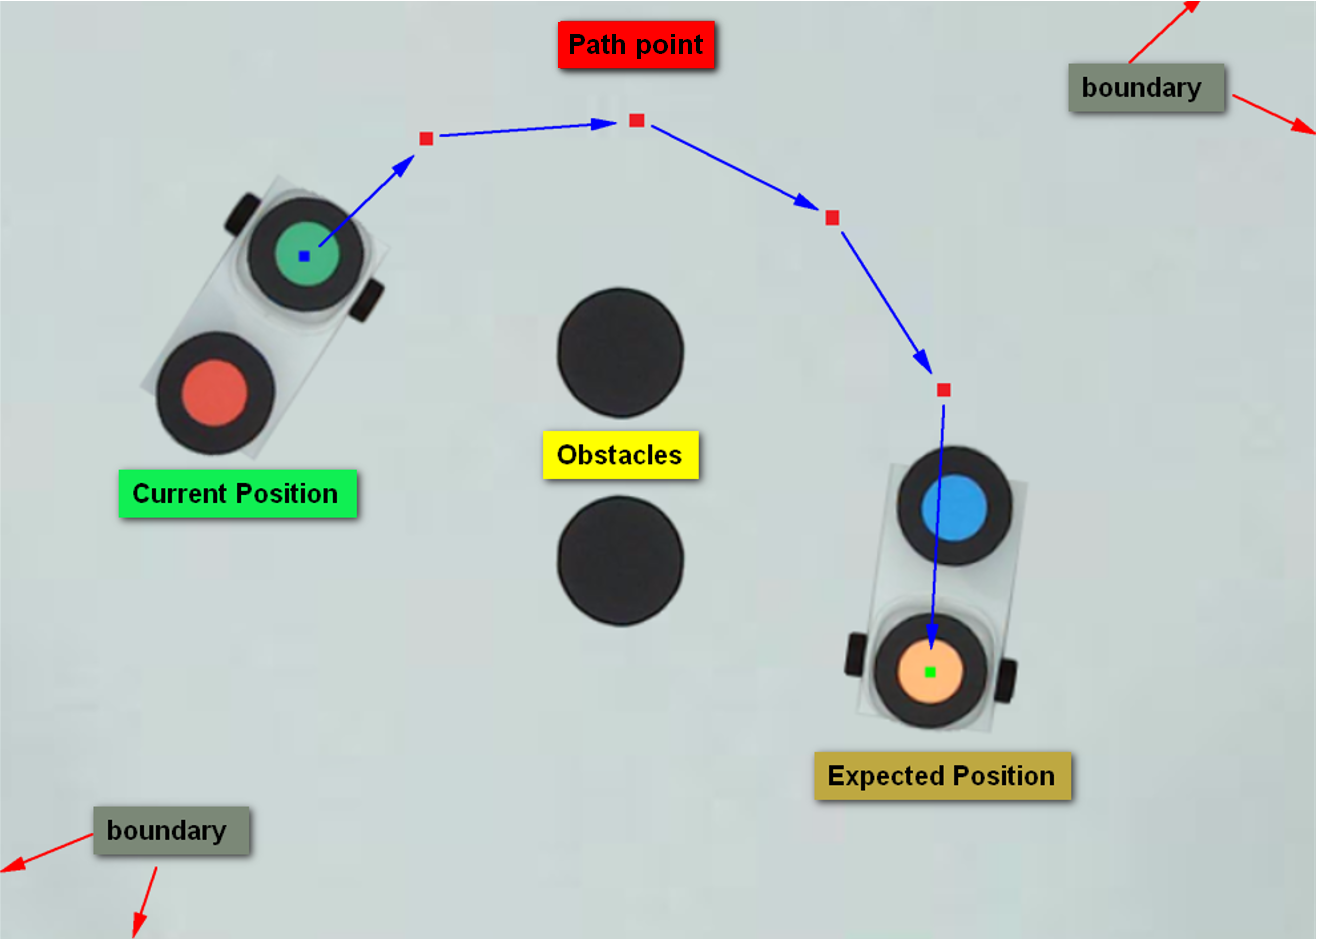
\includegraphics[width=0.6\textwidth]{images/PathPlaningPathPoint.png}
    \caption[How to find the path point]{How to find the path point.}\label{pathpoint}
\end{figure}



\section{The principle and process of ASIA}

According to the tasks and requirements, a novel sampling and iterative based path planning algorithm (called Arc Sampling and Iterative Algorithm(ASIA)) is designed to used in this project.ASIA uses four steps to find and renew a new path point.

\begin{enumerate}
    \item \textbf{Step 1: Get sampling points}\\
    As shown in Figure \ref{samplings}, First, we need to build a body coordinate system. The body coordinate origin is current position , and axis $X$ points the the expected position, and axis $Y$ and axis $X$ intersect at right angles. Second, initialize the value of sampling distance, sampling radian interval and total sampling radian. And get sampling sequence around current position.
    
    \begin{figure}[thb]
        \centering
        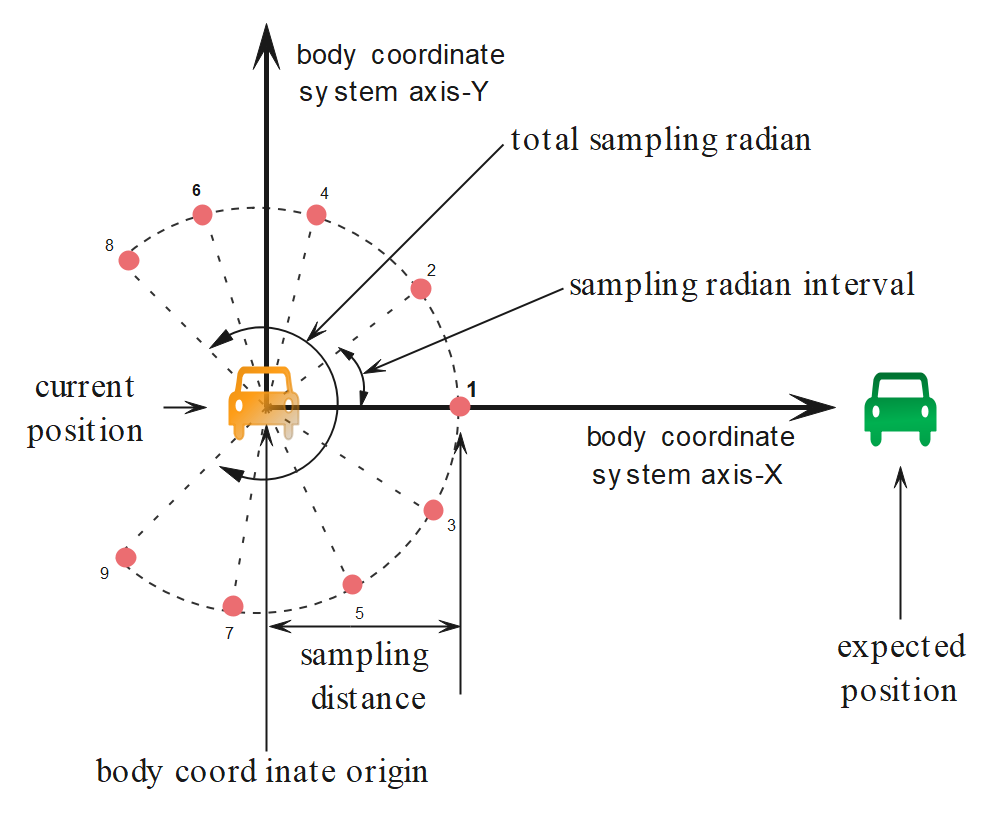
\includegraphics[width=0.5\textwidth]{images/PathPlaningSampling.png}
        \caption[How to find the path point]{How to get sampling points.}\label{samplings}
    \end{figure}
    
    \item \textbf{Step 2: Coordinate transformation}\\
    As seen in Figure \ref{transformation}, In order to get path point sequence in image coordinate systemWe need to translate sampling points from body coordinate system to image coordinate system using rotation matrix after getting sampling points.
    
    \begin{figure}[thb]
        \centering
        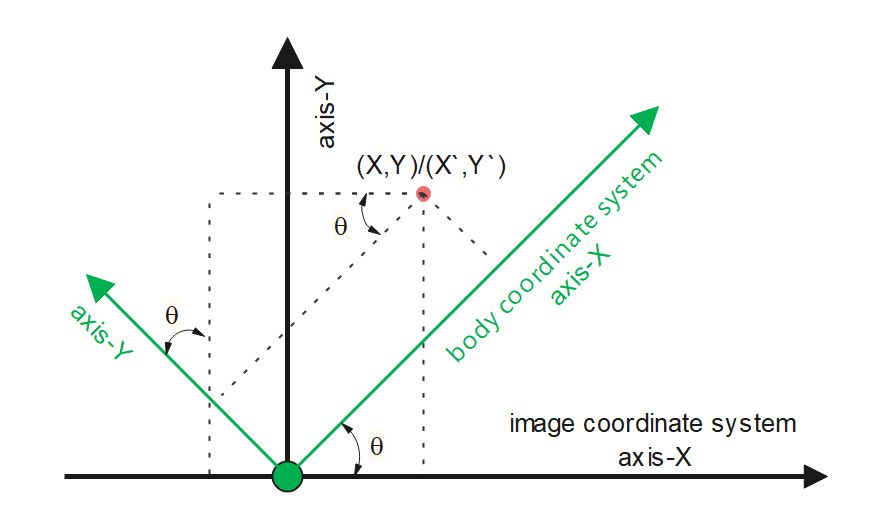
\includegraphics[width=0.5\textwidth]{images/PathPlaningRotationMarix.png}
        \caption[coordinate transformation]{coordinate transformation.}\label{transformation}
    \end{figure}
    
    According to geometric knowledge in figure \ref{transformation}, 
    if the origin position of body coordinate system is $(X_{0},Y_{0})$ in the mage coordinate system, a translation transform need to be added.
    
    \begin{equation}
    \begin{bmatrix}
    X \\Y
    \end{bmatrix}
    = 
    \begin{bmatrix}
    cos\theta & -sin\theta \\sin\theta & cos\theta
    \end{bmatrix} 
    \begin{bmatrix}
    X^{'}\\Y^{'}
    \end{bmatrix} 
    +\begin{bmatrix}
    X_{0}\\Y_{0}
    \end{bmatrix}  
    \end{equation}

    
    \item \textbf{Step 3: Get path point}\\
   As seen in Figure \ref{UpdatePathPoint}, Judging whether the sampling points(here we only show sampling points 1-9) is inside the free space sequentially (not coincide with the obstacle and is located within the image boundary). Once the conditions are met , the sampling points will be taken as the path point and renew current position.
   
        \begin{figure}[thb]
        \centering
        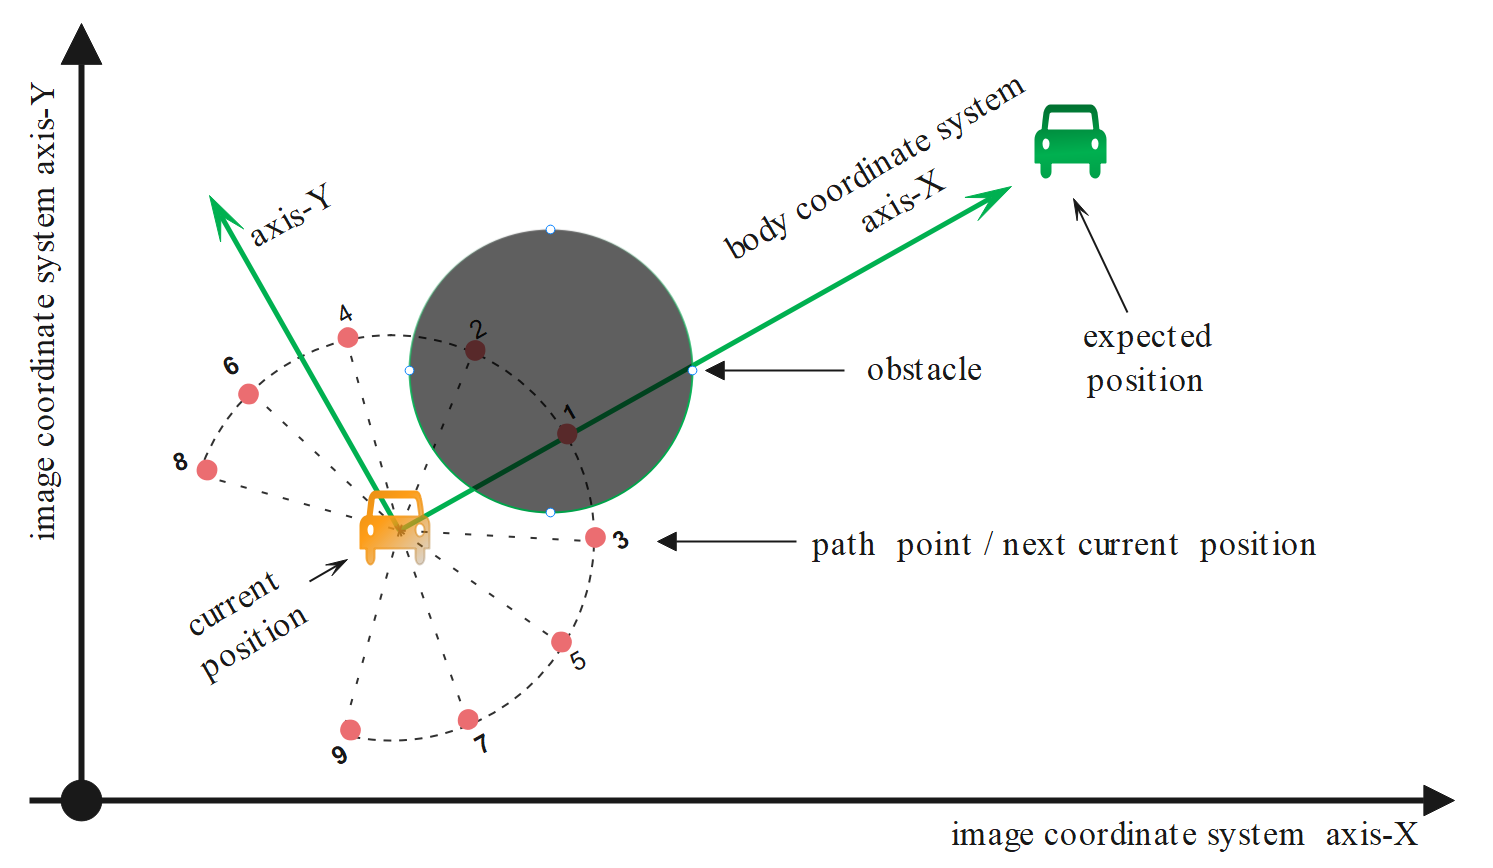
\includegraphics[width=0.5\textwidth]{images/PathPlaningUpdatePathPoint.png}
        \caption[how to get path point and renew current position]{how to get path point and renew current position.}\label{UpdatePathPoint}
    \end{figure}
    
    \item \textbf{Step 4: Iterate to get all of the path point}\\
    Iterate steps 1~3, until the distance between the current position and the expected position is less the the sampling distance.
\end{enumerate}

\section{The implement of ASIA}

There are two parts codes to implement the ASIA. As seen in Figure \ref{part12}, there are four Sub functions Sampling \underline{~} Array, Rotation \underline{~} Array(including TF \underline{~} X and TF \underline{~} Y), Get \underline{~} Angle \underline{~} Rotation and PathTrack to support ASIA. 

\begin{figure}[htbp]
	\centering
	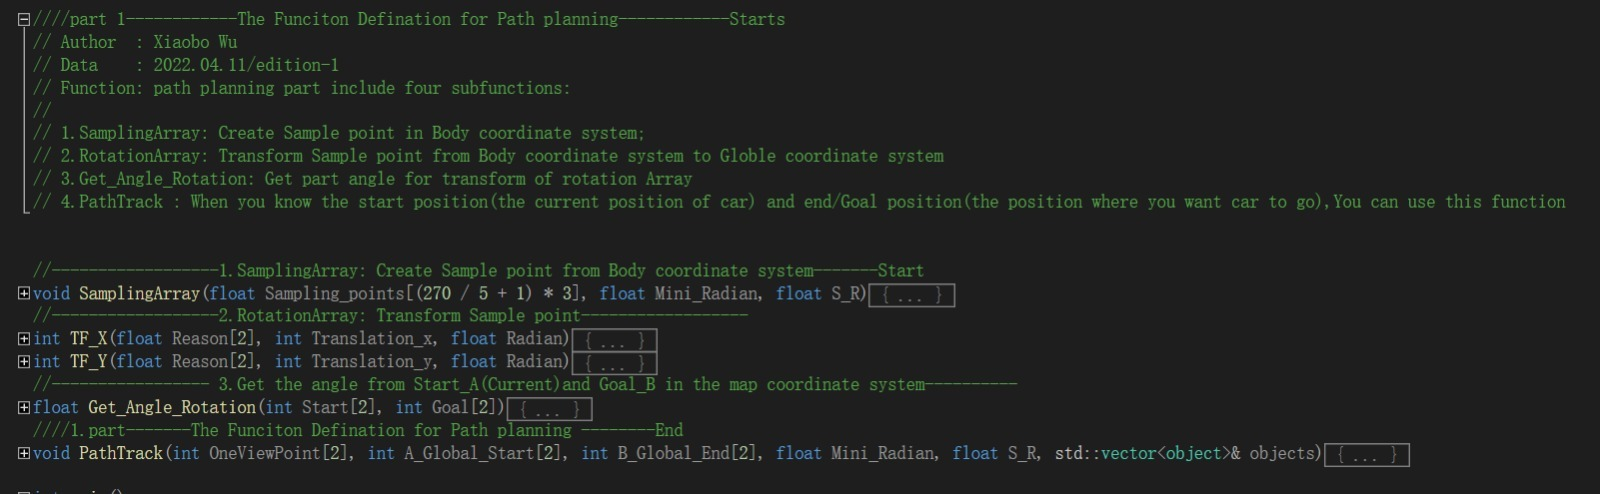
\includegraphics[width =0.9\textwidth]{images/part1.png}

	\caption{The importance of self-robot direction}\label{part12}
\end{figure}


